\newcolumntype{C}[1]{>{\Centering}p{#1}}
\def\TabS#1#2{\small\tabular{#1}\rule[-1.5mm]{0pt}{5mm}{#2}
    \rule[-2mm]{0pt}{2mm}\endtabular}
\def\TabA#1#2#3{\small\tabular{#1}\rule[-1.5mm]{0pt}{5mm}\textbf{#2}\\
    \hline\rule[0mm]{0pt}{4mm}#3
    \rule[-2mm]{0pt}{2mm}\endtabular}
\def\TabB#1#2#3{\small\tabular{c}\rule[-1.5mm]{0pt}{5mm}
    \textbf{{\tiny$\ll$}#1{\tiny$\gg$}}\\
    \hline\rule[0mm]{0pt}{4mm}\tabular{ll}#2\endtabular \\
    \hline\rule[0mm]{0pt}{4mm}\tabular{ll}#3\endtabular
    \rule[-2mm]{0pt}{2mm}\endtabular}
\seticonparams{entity}{
    shadow=false,
    fillcolor=blue!10,
    fillstyle=solid,
    framesep=0pt}

\setcounter{section}{2}
\section{Element Descriptions}
\setcounter{subsection}{-1}
\subsection{Architecture Overview}
\subsubsection{Top Level Design}
It was apparent from the briefing and requirements that the most suitable architecture for the system would be a client-server model. There will be a central server that stores persistent system related data, and performs the majority of the application logic. This server services requests from many client applications that handle user interaction and present information through a graphical user interface. A requirement of the application was also to provide a website as a second source of user interaction, which will be implemented using the central server.

The server and client may be conceptually divided into several modules. For the server, there is the \emph{Database Module} that manages reading from and modifying the persistent application data, the \emph{Logic Module} that handles game and system calculations, and the \emph{Web Interface} group which contains the \emph{API Module} for interacting with client applications, and the \emph{Website Module} for servicing the website HTTP requests. The client will be constructed to include a \emph{Request Module} for contacting the server and interpreting any responses, a \emph{Logic Module} that is aware of relevant aspects of the game state and performs client-relevant calculations, a \emph{Geolocation Module} for interaction with the Google APIs and the GPS sensor, and a \emph{Window Module} for the graphical user interface.

\begin{figure}[h!]
    \centering
    \begin{tabular}{c}
    \entity{server}[\TabA{c}{Centralized Server}{~\\[-3mm]
        \tabular{c}~\\[-10mm]
            \entity{database}[\TabS{c}{Database Module}]\\[8mm]
            \entity{serverlogic}[\TabS{c}{Logic Module}]\\[-3mm]
        \endtabular
        \hspace{5mm}
        \entity{web}[\TabA{c}{Web Interface}{~\\[-3mm]
            \entity{api}[\TabS{c}{API Module}]\\[2mm]
            \entity{website}[\TabS{c}{Website Module}]\\[-3mm] 
        }]\\[-3mm]
    }]
    \hspace{5mm}
    \entity{app}[\TabA{c}{Client Android Application}{~\\[3mm]
        \hspace{-5mm}
        \tabular{cc}
        \tabular{c}~\\[-10mm]
            \entity{request}[\TabS{c}{Request Module}]\\[8mm]
            \entity{applogic}[\TabS{c}{Logic Module}]\\[-3mm]
        \endtabular
        \hspace{2mm}
        \tabular{c}~\\[-10mm]
            \entity{window}[\TabS{c}{Window Module}]\\[8mm]
            \entity{geo}[\TabS{c}{Geolocation Module}]\\[-3mm]
        \endtabular\hspace{-3mm}
        \endtabular
        \\[3mm]
    }]
    \end{tabular}
    {\small
        \ncline[arrowscale=1.5]{<->}{database}{serverlogic}
        \ncline[arrowscale=1.5]{<->}{web}{serverlogic}
        %\ncline[arrowscale=1.5]{->}{database}{web}
        \ncline[arrowscale=1.5]{<->}{api}{request}
        \ncline[arrowscale=1.5]{<->}{request}{applogic}
        \ncline[arrowscale=1.5]{<->}{window}{applogic}
        %\ncline[arrowscale=1.5]{->}{request}{window}
        \ncline[arrowscale=1.5]{->}{geo}{applogic}
    }
    \caption{Data flow of the top level of the system, showing the application and server as clearly separated entities with internal modules that encapsulate distinct functionalities of the system.}
\end{figure}

As \emph{Figure 1} shows, the server and client have a similar overall structure. Both have a main contained logic processing module, a modifiable data source (the \emph{Database Module} for the server and the \emph{Request Module} for the client), and an interface (the \emph{API Module} and \emph{Website Module} for the server, and \emph{Window Module} for the client). This compartmentalisation of processes is intended to make both the server and client subsystems more expandable and maintainable while features are being implemented and testing performed. The interaction between modules is restricted to a small and manageable set of interfaces to help reduce the internal complexity of the system.

\newpage
\subsection{Intermodule Dependencies}
\subsubsection{Database Module}
This module will abstract away interaction with the DBMS (Database Management System), making it possible to easily replace the DBMS used to support different platforms. For the Windows operating system the server will be running on top of the .NET CLR (Common Language Runtime), and will therefore have access to Microsoft's SQL Compact Edition Server. On Unix systems, the server will be using the Mono CLR implementation, and will therefore have to use an alternative DBMS such as SQLite. As well as supporting different DBMS connections and SQL dialects depending on the host system, the Database Module will also provide a simple interface to common SQL operations through the use of code generation. This will reduce the amount of errors produced through the use of poorly constructed SQL statements by delegating the validation task to the debugging facilities provided by the IDE (Integrated Development Environment) used while developing the server.

\begin{figure}[h!]
    \centering
    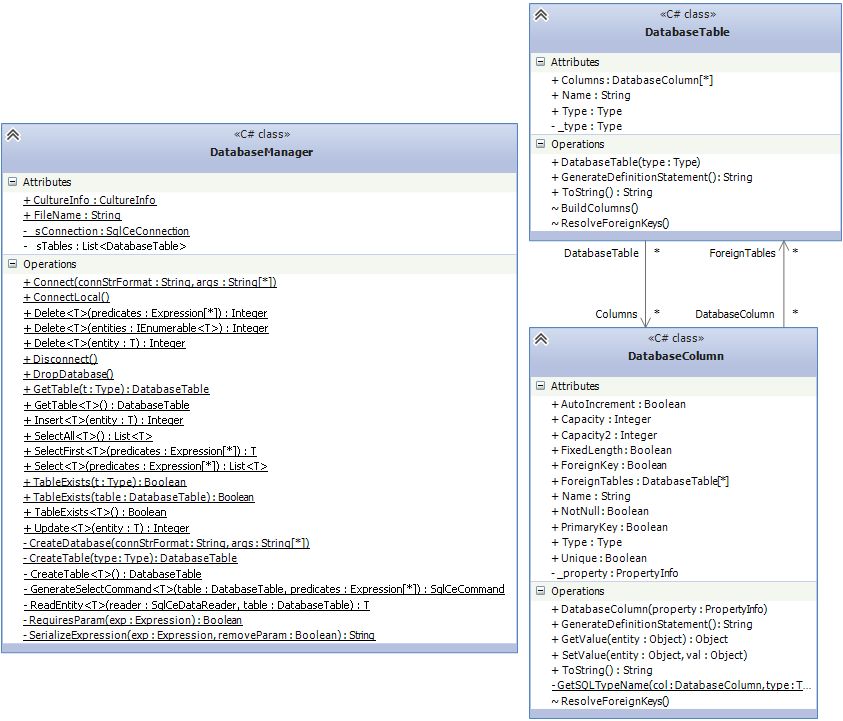
\includegraphics[width=\textwidth]{dbmancd}
    \caption{Class diagram for the main Database Module classes.}
\end{figure}

\subsubsection{Logic Module}
The Logic Module will contain all critical algorithms related to game and overall system state. This will include the operations of account authentication, client location validation, cache attacking, and unit transactions. The module contains a set of core classes that abstract components of the game such as caches and players. Keeping the more intensive calculations in the system separated from the database and interface means they are easier to locate and profile, and unit tests can be produced more simply without having to unnecessarily incorporate unrelated components.

\subsubsection{Web Interface}
This module group is the interface in which incoming HTTP requests are processed and responded to. The requests come in two main categories; website resource requests and API requests. The website resource requests are from users browsing the website and requesting pages or static content such as images. These requests are directed towards the \emph{Website Module}, which processes them and responds with the requested content. API requests are sent by the client application, and will be routed to the \emph{API Module}. These requests are in the form of a command with a series of named parameters, and the response will be sent as a JSON (JavaScript Object Notation) object.

\subsubsection{Website Module}
This submodule of the \emph{Web Interface} handles the delivery of web content such as HTML pages, style sheets, and images. The content is served from a resource directory local to the server program, which is updated during the program's runtime. It also allows dynamic web page generation through the use of inline C$\sharp$ scripts in the source HTML files. These scripts are used as a preprocessing language while constructing the page, so the resulting file sent to a user's web browser has content reflecting the current state of the game and the actions of the user. The inline preprocessor scripting system will be implemented specifically for this project, using code generation and .NET's ``compiler as a service'' facility. The choice to do this instead of simply using PHP or any other pre-existing CGI is so the scripts would have direct access to the server program and its components (this would be true because the scripts are actually contained within the server program itself). This would provide increased performance and would eliminate the need to produce an interface between the CGI and the server.

\subsubsection{API Module}
The second submodule of the \emph{Web Interface} group handles the interpretation and responses to requests from the client application. These requests arrive in the form of a specific command, and the named parameters required by that command. The module contains a class for each command, all extending a general \emph{Request} superclass that provides some facilities common to most requests such as authenticating the requesting user. After the request is processed, an object extending the \emph{Response} superclass is returned by the processing request class. This object is then serialized automatically into a JSON object, which is sent as a reply to the requesting client. The separation of request and response types into classes has the standard benefits of reduced code dependencies and therefore complexity, and also allows requests (or responses) with similar functionalities to extend general abstract classes that implement them. JSON is used as a response format due to its small bandwidth footprint and how trivial it is to parse. It also opens up the possibility of using it with AJAX for the website implementation.

\subsubsection{Request Module}
This module handles the construction and sending of requests to the central server, and then parses and processes the responses given. Each command has a distinct class encapsulating the parameters required and the action to perform with the response. The request classes that have parameters in common extend superclasses implementing those parameters to avoid information duplication and therefore improve maintainability. Other components of the application will, when required, construct a request object instance of the desired type, populate the needed parameters and reference an event handler class to invoke on response arrival, and initiate the request. The request is carried out asynchronously. A flag in the request object will be toggled when a response arrives, and the given event handler triggered. This asynchronous event based pattern is designed to work well with a graphical user interface that must not block execution while waiting for a request, and also allows multiple requests to be performed at the same time.

\subsubsection{Logic Module}
The logic module is where the major processing and validation algorithms of the client application reside. It holds an abstracted model of the game state relevant to the user of the client application, such as data about caches within range of the host device, and profile information about the current user. This module decides what actions the user can perform at each instance in time, and whether an action performed is valid. It also decides what information should be shown to the player, but leaves the details of how it is displayed to the \emph{Window Module}. The components of this module are abstracted for the same reasons as the logic module in the server, to make them easier to locate, unit test, and profile.

\subsubsection{Geolocation Module}
This module has two main purposes, to encapsulate the process of finding the current GPS position of the host device, and to interface with the Google APIs which provide various location based services. The module abstracts the methods used for both functions so as to allow for easy refactoring of the internal implementation, reduce intermodule dependencies, and therefore reduce code complexity. The separation of this set of components from the rest of the system should also make the process of porting the application to other systems such as iPhones easier, since the action of reading from GPS sensors is quite low level and operating system specific and it would be difficult to find all instances of the action if it were spread all over the project.

\subsubsection{Window Module}
The window module will be the largest of the application modules. It encapsulates the graphical user interface, including the presentation of data to the user and the interpretation of user input. The user interface is divided into ``windows'', which are individual views that may be displayed to the client. Examples of windows are the login view, main map display, and the cache attack menu. All windows will inherit from a main abstract superclass that provides the skeleton functionality required by each view. Cleanly separating the application logic from the user interface has numerous benefits; it promotes code decoupling, improves maintainability and the ability to test and profile the code, reduces the amount of information duplication where algorithms are copied for several different views, and means interface layouts and styles can be found and edited with greater ease.
